
\subsection{Estimation of the Lyapunov exponents}\label{sec:sim_LCE}


As mentioned in the previous section, the Boris pusher guarantees a
volume-preserving characteristic. To verify that our simulation's step size is
sufficiently small that the algorithm efficiently preserves volume in phase
space, we employ a concept from chaos theory called the Lyapunov exponents
\citep{Ott2002}. These exponents essentially describe how a basis spanning a $k$-dimensional space changes under subsequent transformations. For simplicity, suppose we have a 1-D trajectory. If the Lyapunov exponent is $\lambda=0$, then the space (distance, in this case) around it evolves as $\exp\qty(n\lambda)=1$
and doesn't contract or expand after $n$ time steps. If $\lambda<0$, the space
eventually reduces to a singular point. This is called an attractor where all
trajectories starting out near this one being considered converges. If
$\lambda>0$, all trajectories originally close together eventually diverge and
become increasingly far from each other. In higher dimensions, these distortions
can be described through the basis elements that span the phase space (see
\cref{fig:ball_expansion}).

\begin{figure}
    \centering
    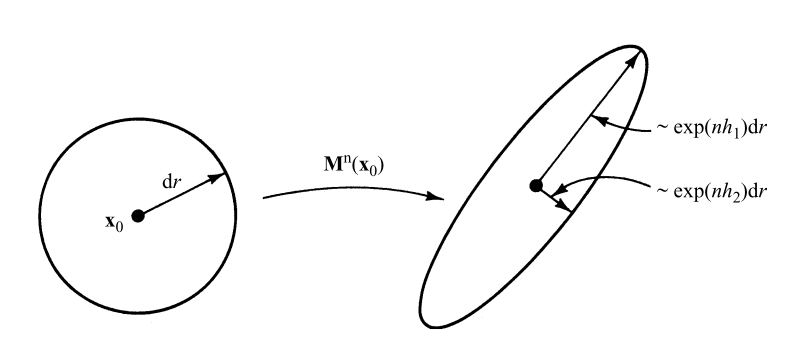
\includegraphics[width=0.8\textwidth]{ball_expansion.png}
    \caption{Distortion of a two-dimensional ball after $n$ time steps.
    $h_1,h_2$ are the Lyapunov exponents in each axial direction spanning the
ball.}
    \label{fig:ball_expansion}
\end{figure}

It requires infinitely many vectors near a point in phase space to compute the
Lyapunov exponents precisely. Thus, one can only estimate the values using a
variety of methods. Here, we shall use a variational approach with Gram-Schmidt
orthogonalization \citep{Benettin1980,Sandri1996}. Given an initial condition to
our ordinary differential equations (ODEs) in the previous section, we can
attach to it a six-dimensional ``ball'' given by a
6x6 matrix, or a set of six 6-D column vectors $U_0=\qty{\vb{u}_j}_{j=1}^6$. This choice of a 6-ball is arbitrary, but the
6-D identity map $\mathbb{1}_6$ is an obvious option. It becomes
$U_1=\vb{M}_0\vdot{U_0}$ after a local expansion $\vb{M}_0=\mathbb{1}_6+\Delta
t\grad\vb{F}_0$ where $\Delta t$ is the step size and $\grad\vb{F}_0$ is the
Jacobian of our ODEs at $n=0$. More details about $\vb{M}$ and $\grad\vb{F}$ can be found in
\cref{sec:expansion_operator}. By the Gram-Schmidt procedure, we can find a
6-D orthogonal basis $W_1=\qty{\vb{w}_j}_{j=1}^6$ from $U_1$. The volume of the
parallelpiped spanned by this new basis is
$V_1(W_1)=\prod_{j=1}^6\norm{\vb{w}_j}$. Now, the definition of the largest
Lyapunov exponent (LCE) after time $t$ is $\lambda=\lim_{t\to\infty}(1/t)\ln
V$ where $V$ is the current volume of the 6-ball. So after $N$ time steps, the
LCE can be approximated as
\begin{equation}
    \lambda=\frac1{N\Delta t}\sum_{n=1}^N\sum_{j=1}^6\ln\norm{\vb{w}_j^n}
\end{equation}
where $t\to N\Delta t$ and $\vb{w}_j^n$ are the basis elements $j$ at time step
$n$. Note the volume is accumulative through time. It is also possible to define separately the Lyapunov exponent in each dimension of the original 6-ball
\begin{equation}
    \lambda_j=\frac1{N\Delta t}\sum_{n=1}^N\ln\norm{\vb{w}_j^n}
\end{equation}
Then the LCE is just the sum of $\lambda_j$ over 6 dimensions. Our calculations
thus involve consecutively computing at each step $n$ the volume of the ball
from $W_n$ and then renormalizing it to measure the expansion of the next
advance. The final result is an accumulation of the volume expansion through $N$
time steps, from which the LCE can be calculated.

